
\documentclass[12pt]{article}
\usepackage[a4paper, margin=.30in]{geometry}
\usepackage{graphicx ,
            wrapfig,
            xcolor, 
            enumerate,
            amsmath,fontenc
            }

\newcommand\headerMe[2]{\noindent{}#1\hfill#2}
\renewcommand{\thesection}{\Roman{section}}

\author{Zakaria HAOUZAN}
\date{\today}

\begin{document}
% headers --------------
\headerMe{Matière : Physique-Chimie}{Professeur : Zakaria HAOUZAN}\\
\headerMe{Unité : Travail Mécanique et Energie }{Établissement : Lycée SKHOR qualifiant}\\
\headerMe{Niveau : 2BAC-SM-X}{Heure : 5H}\\

% ------Content ________
\begin{center}

    \Large{Leçon $N^{\circ} 1 $: \color{red}Ondes mécaniques progressives. }
\end{center}

%\begin{wrapfigure}[10]{r}{0.5\textwidth}
%    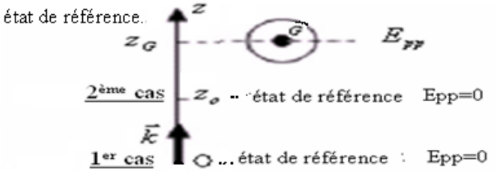
\includegraphics[width=0.5\textwidth]{./img/img00.png}
%\end{wrapfigure}


\section{ Définition d’une onde mécanique : }

On appelle onde mécanique le phénomène de propagation d’une perturbation dans un milieu matériel élastique, sans transport de la matière,mais avec transport d'énergie.
\section{ Ondes longitudinales, transversales, et leurs caractéristiques. }

L'onde est transversale si la déformation du milieu matériel est perpendiculaire à la direction de sa propagation.

L'onde est longitudinale si la déformation du milieu matériel est parallèle à la direction de sa propagation.


\subsection{Propagation d'une onde mécanique le long d'une corde:}
On provoque une perturbation verticale à l'une de ses extrémités d'une corde élastique tendue horizontalement. On constate que la perturbation se propage le long de la corde comme l'indique la figure suivante:
\begin{wrapfigure}[4]{r}{0.5\textwidth}

	
	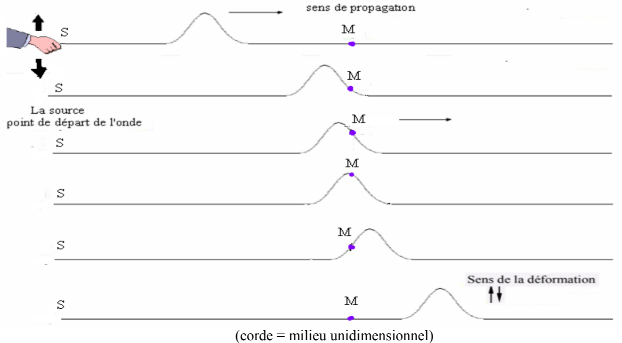
\includegraphics[width=0.5\textwidth]{./img/Corde Propagation.png}
	\caption{Propagation d'une onde mécanique le long d'une corde (corde:milieu unidimensionnel)}
\end{wrapfigure}


\begin{itemize}
	\item La propagation d'une onde mécanique nécessite un milieu matériel (gaz, liquide ou solide).
	\item Dans la cas précédent, la corde qui est milieu de propagation est un milieu matériel, donc il s'agit d'une onde mécanique.
	\item Chaque point M de la corde , lorsque l'onde l'atteint se déplace verticalement (perpendiculairement) à la direction de
propagation : l'onde est donc transversale.
\item Après le passage de l'onde, chaque point M de la corde reste à sa place, donc lors de sa propagation l'onde ne transporte pas la
matière mais elle transporte l'énergie.

\end{itemize}

\begin{wrapfigure}[4]{r}{0.2\textwidth}	
	\vspace{-2cm}
	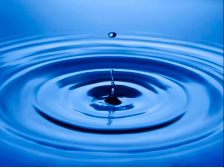
\includegraphics[width=0.2\textwidth]{./img/POM_surface de l'eau.png}
	\caption{Propagation d'une onde mécanique dans l'eau}
\end{wrapfigure}
\subsection{Propagation d'une onde mécanique à la surface de l'eau:}
On provoque une onde circulaire à la surface de l'eau en jetant une pierre dans l'eau (milieu bidimensionnel).

On constate que le morceau de liège placé à la surface de l'eau lorsque l'onde l'atteint se déplace verticalement et il reste à sa
place après le passage de l'onde: donc il s'agit d'une onde mécanique transversale.

\subsection{Propagation d'une onde mécanique le long d'un ressort :}

On comprime quelques spires à l'une des extrémités d'un ressort tendu horizontalement sur une table puis on les lâche brusquement.

\begin{wrapfigure}[4]{r}{0.3\textwidth}	
	%\vspace{2cm}
	\caption{Propagation d'une onde mécanique dans l'eau}
	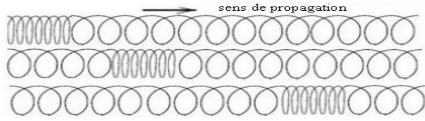
\includegraphics[width=0.3\textwidth]{./img/POM_ressort.png}
\end{wrapfigure}
On constate la propagation de l'onde le long du ressort parallèlement à la direction de propagation, donc il s'agit d'une onde
mécanique longitudinale. (Le ressort=milieu matériel unidimensionnel)


\subsection{Les Ondes sonores :}
\begin{figure}[h]
		\begin{center}
	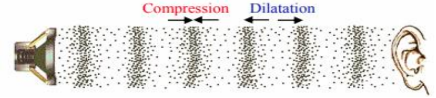
\includegraphics[width=0.3\textwidth]{./img/OndeSonore.png}
	\caption{Onde mécanique longitudinale (onde sonore)}
\end{center}
\end{figure}
\begin{itemize}
\item Le son est une onde mécanique longitudinale tridimensionnelle: sa propagation nécessite la présence d'un milieu materiel ( l'air par exemple mais aussi n'importe quel milieu gazeux, liquide ou solide.)
\item Le son ne se propage pas dans le vide (absence de la matière)..
\item La propagation du son est due à la compression et la dilatation des constituants du milieu de propagation.
\end{itemize}

\subsection{Vitesse de propagation d'une onde :}
La vitesse de propagation d'une onde (nommée célérité) est égale à la distance parcourue au temps mis à la parcourir.












%wfg---------------------------------------------------------------sf 

\section{ Quelques activités du physicien : }

Le physicien observe et étudie les phénomènes naturels et universels tout en cherchant les lois qui les gouvernent.Il
fait des recherches théoriques et expérimentales pour approfondir la connaissance des phénomènes étudiés et mettre
au point de nouvelles méthodes et de nouveaux appareils en contribuant par ses recherches à l'évolution des sciences.

\section{Les questions que se posent les physiciens: }
Plusieurs questions peuvent se poser sur un physicien dans le but de comprendre le fonctionnement des phénomènes
parmi lesquelles on peut citer:
\begin{itemize}
   \item Quelles sont les grandeurs qui permettent d'étudier l'évolution du système étudié ?
   \item Quelles sont les paramètres extérieurs qui commandent cette évolution ?
   \item L'évolution étudiée peut-elle être caractériser par un ou plusieurs temps caractéristique?
   \item Quelle est le rôle des conditions initiales dans l'évolution du système étudié ?
   \item L'évolution étudiée est elle lente, rapide, totale ou limitée , est elle uniforme ou variée? ....

\end{itemize}

      Ensuite le physicien invente des théories et des lois qui expliquent les phénomènes observés tout en se basant sur
l'observation en passant par l'utilisation d'un modèle théorique ou expérimental avant d'extraire les résultats .

Par exemple c'est l'observation de la chute d'une pomme (d’un pommier) qui a conduit Newton à la découverte de la
lois d'attraction universelle.
Newton à son époque s’est posé plusieurs questions :
\begin{itemize}
   \item Qui fait tomber la pomme de l’arbre vers le sol ?
   \item Pourquoi la pomme ne s'éloigne de la terre à tout jamais.?
   \item Pourquoi la Lune ne tombe-t-elle pas elle aussi?
   \item la chute des corps et la révolution de la Lune autour de la terre, obéissent-elles à la même loi physique ?
      \end{itemize}
Ce qui a poussé Newton à découvrir la loi de gravitation universselle suivante:
Tous les corps s'attirent proportionnellement au produit de leurs masses et inversement porportionnelle au carré de la
distance qui les sépare.

\section{Rappel de quelques notions acquis utilisées dans les mesures effectuées par le physicien:}

\subsection{La longueur:}
\subsubsection{Unité de mesure de la longueur: }
L'unité de mesure de la longueur dans le système international est le mètre (m).
Les multiples et les sous multiples du mètre: (tableau de conversion)

\begin{center}
   \begin{tabular}{ |c|c|c|c|c|c|c| }
      \hline
      km & hm & dam & \bf{m} & dm & cm & mm \\
      \hline
        &   &    &  &   &   & \\
\hline
\end{tabular}
On place un seul nombre dans chaque case.
\end{center}
Exemple : 1m  =  100cm et 1cm = 0.01m = $10^{-2}$m

\underline{Autres unités de longueur:}

\begin{itemize}
   \item Le micromètre symbole $\mu$. $1\mu = 10^{-6} m$
   \item Le nonomètre symbole n. $1nm = 10^{-9} m$
   \item Le picomètre symbole p. $1pm = 10^{-12} m$
   \item -L’année lumière al : La distance parcourue par la lumière en une année.\\ $1al = c.\Delta{t} = 3.10^{8}.(365.25 . 24. 3600)= 9.5 10^{15}m$
\end{itemize}

\subsubsection{`Exemples de quelques longueurs :` Le périmètre d’un cercle de rayon R : $P = 2\pi.R$}

\section{La surface:}
\subsection{Unité de mesure de la surface: }
L'unité de mesure de la surface dans le système international est le mètre carré $(m^2)$.
Les multiples et les sous multiples du mètre carré: (tableau de conversion)

\begin{center}
   \begin{tabular}{ |c|c|c|c|c|c|c| }
      \hline
      $km^2$ & $hm^2$ & $dam^2$ & \bf{$m^2$} & $dm^2$ & $cm^2$ & $mm^2$ \\
      \hline
        &   &    &  &   &   & \\
\hline
\end{tabular}
\end{center}
Exemple : $1m^2 = 10^4 cm^2$ et $1cm^2 = 0.0001m^2 = 10^{-4} m^2$


\subsection{Exemples de quelques sufaces:}
\begin{itemize}
   \item Surface d’un disque de rayon R: $S = \pi.R^2$
   \item Surface d’un rectangle S=a.b avec a: longeur , b :largeur
   \item -Surface d’un cylindre de rayon R et de hauteur h: (deux fois la surface de base + la surface latérale) $S = 2\pi.R^2 + 2\pi.R.h$
\end{itemize}
\section{volume:}
L'unité de mesure du volume dans le système international est le mètre cube (m3).
Les multiples et les sous multiples du mètre cube: (tableau de conversion)
\begin{center}
   \begin{tabular}{ |c|c|c|c|c|c|c| }
      \hline
      $km^3$ & $hm^3$ & $dam^3$ & \bf{$m^3$} & $dm^3$ & $cm^3$ & $mm^3$ \\
      \hline
        &   &    &  &   &   & \\
\hline
\end{tabular}
   \begin{tabular}{ |c|c|c|c|c|c| }
      \hline
       $hL$ & $daL$ & \bf{$L$} & $dL$ & $cL$ & $mL$ \\
      \hline
        &   &    &  &   &    \\
\hline
\end{tabular}
\end{center}

Exemple : $1m^3 = 10^6 cm^3$ et $1cm^3 =  10^{-6} m^3$

Remarque: Pour mesurer le volume des liquides on utlise souvent le litre symbolisé par (L)
Les multiples et les sous multiples du litre: (tableau de conversion)
\begin{center}

\end{center}

Exemple : $1m^3 = 10^3 $L et $1L =  1000 mL$ 



\end{document}

